\section{Materials and Methods}
\subsection{Public sources and study period}
The source study used official, account-free NOAA services. Satellite files were selected from \url{https://manati.star.nesdis.noaa.gov/UHR_COASTAL/}, without redirects or credentials. A listing inventory of 1,232 requests was collected on 4 November 2026 between 06:39:16 and 07:22:46 UTC and bound to the protocol by cryptographic digests. Listing metadata defined the candidate universe; they did not establish each file's original dissemination time, continued availability, or processor version.

The study interval was 17 June 2026, 00:00 UTC, through 4 November 2026, 00:00 UTC, with the final endpoint excluded. Five consecutive 28-day blocks began on 17 June, 15 July, 12 August, 9 September, and 7 October. The eight evaluation stations were 41047, 42001, 42035, 42036, 42056, 44008, 44014, and 44020. The four development stations were 41008, 42002, 42039, and 44027. Figure~\ref{fig:stations} places the reported station coordinates in their geographic context; the roles and original selection labels are listed in Supplementary Table~S1.

Station selection used official static metadata and time coordinates. Within each region, eligible stations were divided into four latitude-rank bins, and a stable salted hash selected one evaluation station per bin. The remaining candidates were repartitioned into two bins per region; a different salt selected disjoint development stations. This separation was introduced in the version-4-to-4.1 protocol repair before recorded wind-outcome access. No wind speed, wind direction, or outcome-side ancillary variable was used in the selection.

\begin{figure*}[!t]
\centering
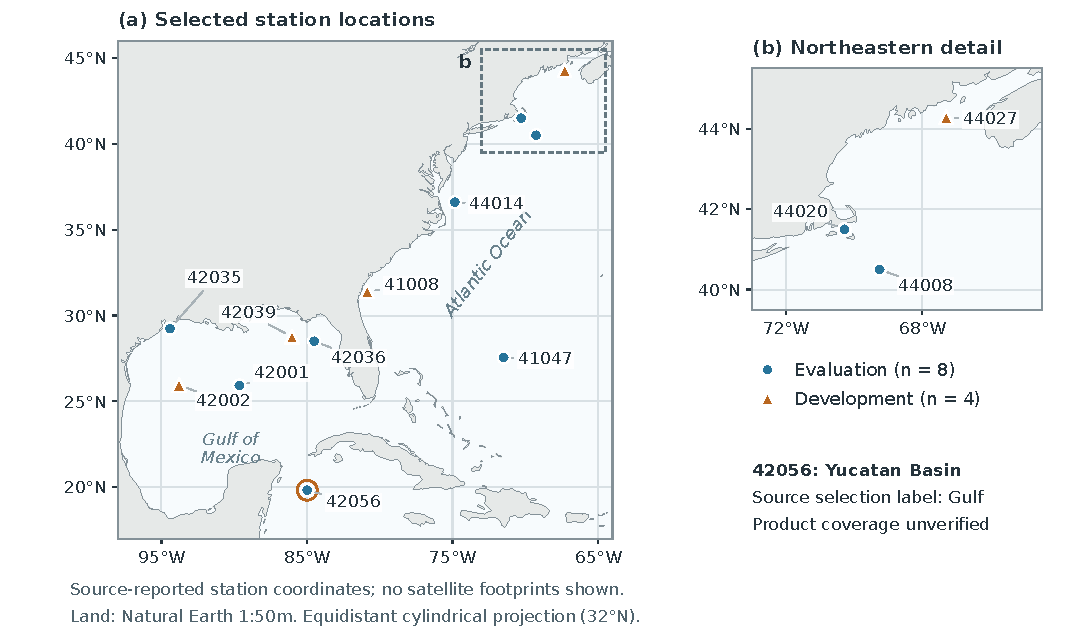
\includegraphics[width=\textwidth]{figures/station_map.pdf}
\caption{Reported station locations and study roles. Coordinates are transcribed from the source study's period-median deployment record. The northeastern inset separates nearby stations. Land outlines use Natural Earth at 1:50 million scale \cite{naturalearthland}. This is a geographic context map, not a satellite-coverage map. Station 42056 retains the original Gulf selection label; its association with the selected product footprints remains unverified.}
\label{fig:stations}
\end{figure*}

\subsection{File selection and alternate rounds}
Eight file strata crossed the Atlantic and Gulf product sectors (\texttt{ec}/\texttt{gc}), MetOp-B and MetOp-C, and ascending and descending passes. Each stratum was divided into 12 equal time bins. One salted-hash minimum per stratum and time bin supplied the 96 primary files.

A logical satellite observation was identified by platform/pass prefix, sensing time, orbit, and sector. Only base variants were eligible. Revisions were resolved by highest revision and then lexical stem order; the filename was not treated as evidence of processor version. A separate salted ordering of nonprimary observations supplied four alternate rounds, each containing one file from every stratum. Thus the entire selectable set was fixed at 128 files before opportunity counts determined how many rounds to activate.

All active extracts had to reach a final processing state before a capacity decision. Counts could trigger the next whole round, but could not change its order or select individual files within it. Development-station counts were report-only and could neither activate a round nor satisfy the evaluation gate. Complete rounds maintained balanced increments across the eight strata. The policy was a control on adaptive file choice, not an attempt to maximize yield per downloaded byte.

\begin{table*}[!t]
\caption{Fixed benchmark design and capacity rule}
\label{tab:design}
\centering\small
\begin{tabularx}{\textwidth}{@{}p{0.19\textwidth}Y Y@{}}
\toprule
Element & Specification & Meaning for this audit \\
\midrule
Study population & 128 selectable files; 8 evaluation and 4 development stations & Only evaluation opportunities contribute to the capacity gate. \\
File strata & 2 sectors $\times$ 2 platforms $\times$ 2 pass directions & 96 primary files from 12 time bins per stratum. \\
Repair policy & Four ordered rounds of 8 alternate files & Whole rounds only; no file substitution or reordering. \\
Period & 17 June--4 November 2026, UTC; final endpoint excluded & Five consecutive 28-day blocks; 40 evaluation cells. \\
Counting unit & Unique station--logical-observation pair & A $5\times5$ neighborhood contributes at most one opportunity. \\
Spatial/candidate rule & Center within 12.5 km; at least 2 valid ambiguity candidates & Passing denotes protocol eligibility, not verified wind accuracy. \\
Capacity rule & At least 400 total and 8 per station--block cell & Both conditions must pass before outcomes can be opened. \\
Acquisition limits & 10,000,000,000 new science bytes; at most 2 transient raw files & 128 selected files are a bounded design, not an archive census. \\
Specification status & Repository-local freeze before recorded outcome access & No public preregistration; the later audit is exploratory. \\
\bottomrule
\end{tabularx}
\end{table*}

\subsection{Opportunity definition and quality rules}
An opportunity was one unique pair of station identifier and logical-observation key. Deterministic nearest-center selection had to locate a protocol-valid retrieval coordinate within 12.5 km of the station. Its center-pixel time had to fall within the study interval and a specified block, and a verified predictor neighborhood had to be available. Each extract contained a same-file, same-pass $5\times5$ neighborhood; out-of-bounds cells were invalid. The 25 pixels did not create additional opportunities.

Each retrieval cell could contain up to four wind-ambiguity candidates, of which at least two had to be valid. Invalid coordinates, land, ice, numerical-weather-prediction ice, missing pixel time, candidate-shape mismatch, an out-of-range selected index, and unresolved direction semantics were grounds for rejection. NOAA quality-control, rain, and anomaly-filter flags were retained as descriptors rather than used to exclude cases. Their presence therefore did not directly reduce the opportunity count. Conversely, the processing label \texttt{extract\_valid} indicates compliance with these predictor rules, not an assessment of retrieval accuracy.

If several records represented the same station--observation pair, their deterministic order was distance, absolute time difference from file sensing time, file SHA-256 digest, center row, and center column. The audit materialized all 40 evaluation station--block cells, including zeros. The 30-minute buoy-collocation tolerance specified for the later performance study was not used in this predictor-only count.

\subsection{Capacity gate and stopping condition}
Let $N_{s,b}$ denote the number of distinct opportunities at evaluation station $s$ in block $b$, and let $N_{\mathrm{eval}}$ be their total. With eight evaluation stations $\mathcal{S}$ and five blocks $\mathcal{B}$, the gate passes only when
\begin{equation}
N_{\mathrm{eval}}\geq400
\quad\text{and}\quad
\min_{s\in\mathcal{S},\,b\in\mathcal{B}}N_{s,b}\geq8.
\label{eq:gate}
\end{equation}
The rule is evaluated after the primary files and after every complete alternate round. An intermediate failure activates the next round. Failure after round 4 stops the workflow with \texttt{FAIL\_EXHAUSTED} and leaves B1 unauthorized.

The planned downstream analysis required at least 320 cases overall and six per cell. The predictor thresholds of 400 and eight therefore allowed 20\% aggregate and 25\% cell-level attrition before those minima would be violated. These margins explain the relationship between the two configured gates. They were not derived from a statistical power or precision calculation.

\subsection{Processing states and transfer accounting}
Each of the $128\times12=1{,}536$ station--file combinations required one final state: a valid extract, fewer than two valid candidates, no spatial overlap under the specified rule, or invalid time. The corresponding stored labels were \texttt{extract\_valid}, \texttt{fewer\_than\_two\_valid\_candidates}, \texttt{no\_overlap}, and \texttt{time\_invalid}. These labels describe the workflow's disposition of a record; they do not identify a physical cause.

Final-key accounting also required one selection record and one transfer record per selected source, and one predictor-case record per evaluation opportunity. Earlier transfer attempts remained linked to their parents. Downloaded objects were distinguished from preexisting geometry evidence reused by digest. Probe bytes were counted separately, and no transient raw download could remain when the transaction closed.

The inventory and extract denominators describe different objects. The 1,232-request listing inventory includes 560 date-prefix requests within the study interval. Of those 560, 141 carried the combined label \texttt{public\_endpoint\_empty\_or\_not\_backfilled}. This label does not distinguish absence of an observation from the state of the public listing or backfill. The station--file tables, in contrast, include every selected file paired with every station in the relevant role; their denominators are not estimates of expected physical overpasses.

\subsection{Deterministic replay and integrity checks}
The replay read eight declared inputs: the source opportunity report, transaction receipt, selection ledger, transfer ledger, station-extract manifest, station-role manifest, evaluation-case Parquet, and a tree of 128 per-file predictor receipts. It also bound six evaluator artifacts: the inherited opportunity, terminal-state, and pre-outcome-freeze contracts, together with the later audit commitment, claim map, and replay specification. File or tree digests were checked before parsing.

The replay rejected network locations, path traversal, undeclared inputs, outcome-like paths, and prohibited outcome fields. From the allowed inputs it recomputed file membership, station roles, block identities, opportunity keys, the zero-filled count matrix, stage contributions, processing-state distributions, final-key closure, transfer-attempt parent chains, byte totals, raw-file disposition, and Parquet properties. It also checked the explicit outcome-read counters and the different meanings of the source and audit gates. Thirteen integrity checks had to pass without disagreement.

The three final outputs had to be absent before execution. A lock protected the transaction; the comparison ledger and narrative were committed before the final JSON receipt. Bound inputs were checked again before the receipt was written, and output bytes were checked afterward. This procedure checks repository-local consistency and detects incomplete output states. It does not establish power-loss atomicity or isolation from an unrelated process changing files concurrently.

\subsection{Audit scope and statistical treatment}
The original record contains one eligible version-5 replay run, identified as \texttt{RUN-R1-V5-B0-FEASIBILITY-REPLAY-A1}. It was linked to both audit claims and verified by a non-owner within the same research environment. The subsequent result audit included that run and excluded none. It recorded agreement for protocol, metrics, outcome accounting, provenance, and continuity, but failed its formal independence check because the audit shared the source implementation and repository context. The resulting classification was exploratory support rather than independent confirmation.

For the descriptive acquisition profile, each alternate round's marginal yield was its additional evaluation opportunities divided by the volume of additional transferred science data in decimal GB. This ratio summarizes the realized sequence and does not compare unexecuted policies.

All reported counts enumerate the selected universe. They are not estimates obtained from a probability sample of the wider NOAA archive. We therefore report neither confidence intervals nor significance tests. Generalization to other file selections, stations, or periods requires a separately specified population and analysis design. Supplementary material lists the execution commands and artifact paths reported for the source study. Independent reproduction is outside the evidence provided here.
